% !TeX spellcheck = en_US
\documentclass[12pt, a4paper, titlepage]{book}
\usepackage[a4paper, margin=3cm]{geometry}
%\setlength{\parindent}{0pt}
%\setlength{\parskip}{14pt plus 5mm minus 4mm}

\usepackage[utf8]{inputenc}% erm\"oglich die direkte Eingabe der Umlaute 
\usepackage[T1]{fontenc} % das Trennen der Umlaute
\usepackage[english]{babel}
\usepackage[breaklinks,hidelinks]{hyperref}
\usepackage{xspace}
\usepackage{lmodern}
\usepackage{textcomp}
\usepackage{graphicx}
\usepackage{color}
\usepackage{caption}
\usepackage{comment} 
\usepackage{listings}

\usepackage{amssymb}
\usepackage{amsmath}

% set date format
\usepackage[style=iso]{datetime2}
%\usepackage[yyyymmdd]{datetime}
%\renewcommand{\dateseparator}{--}

% shortcuts
\newcommand{\jws}{JWS~Online\xspace}
\newcommand{\django}{Django\xspace}
\newcommand{\sedml}{SED-ML\xspace}
\newcommand{\mathml}{MathML\xspace}
\newcommand{\simexp}{simulation experiment\xspace}
\newcommand{\fairdom}{Fairdom\xspace}
\newcommand{\mathematica}{Mathematica\xspace}
\newcommand{\json}{JSON\xspace}
\newcommand{\numl}{NuML\xspace}
\newcommand{\combine}{COMBINE\xspace}
\newcommand{\ca}{\combine~archive\xspace}
\newcommand{\sbml}{SBML\xspace}
\newcommand{\cellml}{CellML\xspace}
\newcommand{\xml}{XML\xspace}
\newcommand{\rdf}{\xml~RDF\xspace}
\newcommand{\owl}{OWL\xspace}

\newcommand{\masymos}{MaSyMoS\xspace}
\newcommand{\bives}{BiVeS\xspace}
\newcommand{\comodi}{COMODI\xspace}
\newcommand{\neoj}{neo4j\xspace}

\newcommand{\sysbio}{System Biology\xspace}
\newcommand{\rest}{REST\xspace}  % like in REST interface

% TODO command
\newcommand{\todo}[1]{{\color{red} TODO: #1}\\}
\newcommand{\dw}[1]{\textbf{\color{green} DW: #1}\\}

\title{Conception and Prototype Implementation of a storage solution for Models with multiple Versions}
\author{Martin Peters\\[12pt]
	\small Department of Systems Biology and Bioinformatics\\
	\small University of Rostock}
\date{\today}

\begin{document}
	\maketitle
	\tableofcontents
	
	\chapter{Introduction}
	% comment command for Dagmar (defined in shortcuts.tex)
	%\dw{This a is comment from Dagmar}
	\section{Motivation}
- Reproducibility
	- \sedml is useless, when model changes
- Transparency
- Tracking differences
	- what has changed
	- who has changed it
	- oxford2012 + first bives paper
	
- Doing analysis of the evolution of a biological model
- provide a comprehensive repository of biological models and their history
- discover similarities and differences in the development of model through Ontology crosslinking
- Motivation out of koehn2008 \cite{Kohn2008}

\section{Goals}
- extend an existing database to store multiple versions of one model in it
- semantically connect the versions
- store idfferences to allow for efficient analysis
- \todo[talk about possible results]
	
	\chapter{Difference detection and its challenges for System Biological Models}
	% !TeX spellcheck = en_US
\section{Data formats for System Biology models}
	\label{sec:background:formats}
	
	At the time this thesis is written, there are two major formats to encode models in \sysbio. With combined over 3237 models in 14439 versions openly available\footnote{\url{http://most.sems.uni-rostock.de/}}, \sbml and \cellml encode a large amount of accessible models in \sysbio.
	Both were independently developed, but serve the similar purpose of "support[ing] basic biochemical network models" \citep{Cuellar2003}. Further they use the eXtensible Markup Language \citep{Bray1998} (\xml) as base format, which makes them human readable and enables the use of generic \xml tools and standards \citep{Cuellar2003,Hucka2003} like MathML \citep{Carlisle2003}, XLink \citep{DeRose2010}, and \rdf \citep{Lassila1998}.
	
	Even with serving similar purpose \sbml and \cellml are structured quite different.
	\cellml, for instance, defines a broader scope and features a modular structure, which allows to describe "complex interconnected cell models" \citep{Cuellar2003}.
	The basic design of \cellml represents a "network of interconnected components" \citep{Cuellar2003}, which may contain \emph{variables}, and mathematical \emph{equations}. These \emph{equations} determine the behavior of a \emph{component} within a model.
	A \emph{component} is meant to represent a biochemical reaction with it reactants and products, which are represented by \emph{variables}.
	To interlink individual \emph{components} different variables are mapped between them. These mappings are organized in so called \emph{connections}, which are defined between two \emph{components}. Additionally \emph{connections} have to be unique for to given \emph{components}, which means that all mappings between two \emph{components} have to be listed in a single \emph{connections}. (cf. \citet{Cuellar2003})
	
	In contrast to the generic concept of \cellml, defines \sbml more specific design elements.
	A \sbml \emph{compartment} provides a logical or biological container for \emph{species} and \emph{reactions}.
	
	
	\begin{comment}
	\begin{itemize}
		\item formats
		\subitem SBML
		\subitem CellML
		\subitem \sedml
		\item everything in XML
		\item semantic annotations
	\end{itemize}
	\end{comment}

\section{Detecting differences in Version Control Systems}
	\label{sec:background:diff}
	
	\subsection{Unix Diff}
	\label{sec:background:diff:unix-diff}
	The essential building block for each Version Control System (VCS) is an algorithm or tool to detect differences between two or more versions, because just storing each version completely is a waste of storage and bandwidth. Further processing change sets enables the system to automatically merge different development branches and therefore making collaboration more efficient.
	
	Nowadays most general-purpose VCS use the \emph{diff} utility, developed as part of UNIX \citep{Chacon2014,OSullivan2009,Collins-Sussman2004}. It is based on the Hunt-McIlroy algorithm, which tries to solve the longest common subsequence problem for two files \citep{Hunt1976}.
	The result is a report of all differences between two files, "expressed as a minimal list of line changes to bring either file into agreement with the other" \citep{Hunt1976}.
	
	\begin{comment}
	\begin{itemize}
		\item Based on solving the longest common subsequence problem
		\item "The program diff reports differences between two files, expressed as a minimal list of line changes to bring either file into agreement with the other" \citep{Hunt1976}
		\item "The central algorithm of diff solves the ‘longest common subsequence problem’ to find the lines that do not change between files" \citep{Hunt1976}
	\end{itemize}
	\end{comment}
	
	\subsection{XML Diff}
	\label{sec:background:diff:xml-diff}
	The problem with the default algorithm used by general-purpose VCS (cf. Section \ref{sec:background:diff:unix-diff}) is, however, that it does only distinguish between text based and binary formats. Hence making none or very little assumptions about the underlying document. Therefore it fails to recognize features, specific to the format. These line-base algorithms tend to be problematic especially for \xml, since line breaks can be neglected, without changing the encoded information. \citep{Ronnau2005}
	
	It can be concluded, that the usual diff algorithm is too fine granular, since it also reacts to changes in the encoding. \xml is represented as hierarchical tree structure and thus it is possible to detect changes based on their position in the tree, rather than a line-number \citep{Wang2003,Chawathe1996,Cobena2002}.
	This can be archived by identifying unchanged subtrees and map them between source and destination version. Going out from those mapped tree, more and more nodes can be matched, under consideration of ancestors, descendants, and labels. Also changed attributes or text-nodes need to be treated differently \citep{Cobena2002}.
	
	\todo{add ref to both examples XyDiff + the other one?}
	
	\begin{comment}
	cf. Cobena2002 \citep{Cobena2002} and \citep{Waltemath2013} in section 2.2.1
	Chawathe et al., 1996 \citep{Chawathe1996}
	\begin{itemize}
		\item "With flat information deltas may be represented simply as sets of tuples or records inserted into, deleted from, and updated in relations. In hierarchical information, we want to identify changes not just to the 'nodes' in the data, but also to their relationships." \citep{Chawathe1996}
		\item "General-purpose version control systems attempt to handle any kind of document and thus make no assumptions about the underlying document format. Usually, those systems distinguish between binary documents and text documents. Appropriate diff algorithms are employed to detect changes between two versions of a document. Those diff algorithms are either line based (for text documents) or byte based (for binary documents). General-purpose version control systems provide good control for line-organized text documents such as source code or latex documents. For XML documents, where the organization into lines can be neglected, 2 line-based version control is inappropriate." \citep{Ronnau2005}
		\item requirements
			\subitem "Within a delta, the exact location of the change must be identified." \citep{Ronnau2005}
			\subitem "XML Structure Information. An XML document is generally a hierarchically structured document, and can be represented in a tree structure. However, an XML document has other features that distinguish it from a general labeled tree. X-Diff introduces the	notion of node signature and a new matching between the trees corresponding to the two versions of a 	document. Together, these two features are used to find the minimum-cost matching and generate a minimum-cost edit script that is capable of transforming the original version of the document to the new version." \citep{Wang2003}
			\subitem "Unordered Trees. Since XML documents can be represented as trees, the change detection problem is related to the problem of change detection on trees." \citep{Wang2003}
		\item "It [the algorithm] tries to detect (large) subtrees that were left unchanged between the old and new versions. These are matched. Starting from there, the algorithm tries to match more nodes by considering ancestors and descendants of matched nodes and taking labels into consideration. Our algorithm also takes advantage of the specificities of XML data. For instance, it knows of attributes and attribute updates and treat them differently from element or text nodes. It also takes into account ID attributes to match elements." \citep{Cobena2002}
	\end{itemize}
	\end{comment}
	
	\subsection{BiVeS}
	\label{sec:background:diff:bives}
	\todo{use the terms source and destination document}
	Continuing on the problem described, in section \ref{sec:background:diff:xml-diff}, the same issue with \xml documents and normal delta algorithms scales to more specific documents and \xml delta algorithms. In this case we look at \xml encoded biological models, either using \cellml or \sbml. Even though algorithms described in the prior section are treating \xml documents as trees, they still lack deeper understanding of a biological model for instance. \bives addresses this issue by building upon XyDiff (cf. section \ref{sec:background:diff:xml-diff}), and by incorporating additional features specific to system biological models, like ontology links, attribute references, and special parts of the model, which are treated atomically \citep{Scharm2015}.
	
	\bives tries to match subtrees of two models, by calculating a hash and a weight for each possible subtree, whereby the weight is always greater than the weight of its children.
	First, the identifying attributes (\xml id attribute and links to bio-ontologies) are used to create a first mapping. Second, this initial mapping is propagated upwards in the document's structure, meaning the connection of a node's children are traversed depth-first and the mapping of these children is suggested for their parents, except if tag-names mismatch. Among the suggested candidates, the most promising mapping is chosen.
	Third the initially generated hashes are used to map remaining subtrees. A priority queue maintains the processing order, so the larger subtrees are mapped first.
	As last step the quality of the mapping is improved by examining the network structure top-down. Each unmapped child is compared to unmatched children in the opposite document and new mappings are created with a maximum distance of $0.9$. This ensures, that completely unrelated nodes are not connected.
	Additionally domain specific mapping rules are in place to apply different strategies for specific characteristics. For instance, certain parts of a model document are treated as atomic units. Whereby different changes in the hierarchical structure are forbidden, which means, that these mappings are unlinked. This is a crucial step, leading to better quality results, when compared to standard \xml delta algorithms.
	
	Finally the different change types are distinguished, by comparing the mappings. An \texttt{insert} is for instance only present in the destination model, but has no mapping to the source model. In contrast a \texttt{delete} can only be found in the source model, certainly not in the destination.
	However these two are called unmapped changes, hence they are identified by the missing link. Opposed to this kind of changes, mapped nodes lead to either an \texttt{update}, \texttt{move}, or no change.
	A \texttt{move} is specified as a case, in which the node is present in both source and destination, but either the parents are not connected, or the order of their siblings is different. An \texttt{update}, however, happens, when the value of an attribute, the content of a text node or the tag name has been alternated.
	
	The resulting \xml delta can be outputted in several formats, including \xml, dot\footnote{\todo{link to graphviz}}, GraphML\footnote{\todo{}}, \json, or as text reports in several markup languages.
	In this work I, will only focus on the \xml output, since it is easy to process and the latest version of \bives also includes \rdf annotations linking to \comodi (cf. section \ref{sec:background:onto:comodi}) \citep{Scharm2015}.
	\todo{include a nice bives figure}
	
	\begin{comment}
	\begin{itemize}
		\item benefits of XyDiff compared to unix-diff
		\subitem problems with XML
		\subitem no deeper "understanding"
		\item cf. \citep{Waltemath2013} (Oxford 2012), \citep{Scharm2015}
		\item algorithm (list of quotes from \citep{Scharm2015})
		\subitem two versions of an XML-encoded model are translated into an internal tree structure. For every node n in the tree, a hash sum n r and a weight n x are calculated 
		\subitem The weight of a node is thus always greater than the weight of its children. As such, the weight represents the size of the corresponding subtree 
		\subitem The hash sum of a node n represents the signature of the subtree rooted at n 
		\subitem While n r unambiguously defines the subtree rooted in n, n r does not need to be unique among all nodes in the tree. Thus, if n r ¼ m r then the subtrees in n and m are identically equal 
		\subitem First, nodes are being mapped with respect to their identifiers 
		\subitem id attributes in the XML documents serve as identifiers. In addition, we also evaluate biological identifiers, specifically links into bio-ontologies 
		\subitem Second, the initial mapping is propagated upwards into the trees. 
		\subitem The connections of a node’s children are evaluated in a depth-first traversal of T 2 . If a node n in T 2 is connected to a node m in T 1 then a mapping of parent ðnÞ to parent ðmÞ is suggested 
		\subitem If, in contrast, n is not connected, we examine the candidates that were previously suggested by the connections of n’s children. 
		\subitem Candidates which have a different tag name than n and candidates which al- ready have a connection are neglected. 
		\subitem Among the remaining candidates, the algorithm chooses the one that received the best suggestions and connects it to n 
		\subitem Third, the algorithm makes use of the initially computed signatures and maps nodes of T 2 on nodes of T 1 
		\subitem A priority queue U is maintained to sort the nodes of T 2 based on their weights. Initially, U only consists of the root node of T 2 . 
		\subitem Unless U is empty, the algorithm repeatedly removes node n 2 U  T 2 with the biggest weight, which represents the biggest subtree in the queue 
		\subitem Fourth, the algorithm improves the quality of the mapping by examining the network structure of T 1 and T 2 in a top-down approach. For every mapping n 2 T 2 on m 2 T 1 , it compares unmatched children of n and m to find missed mappings 
		\subitem The algorithm evaluates the matrix greedily and adds new mappings up to a maximum distance of 0.9. Thus, nodes which have nothing in common will not be connected 
		\subitem Additional mapping rules capture the domain characteristics of the processed data. Following the current specifications for SBML and CellML, we prohibit certain changes in the hierarchical tree of document nodes. Specifically, we treat parts of the model as atomic con- structs for which we define restrictions on possible network operations 
		\subitem This step is a major reason why our algorithm outperforms standard XML diff algorithms. 
		\subitem insert if an entity is present in T 2 but absent in T 
		\subitem delete if an entity is present in T 1 but absent in T 
		\subitem move if a node is present in both documents, but either (i) the parents in the corresponding trees are not connected or (ii) the parents are connected, but the sequence of their siblings has changed 
		\subitem update if the value of an attribute, a text node's content or the tag name of a node was modified
		\subitem After the mapping, we distinguish two types of nodes: mapped nodes and unmapped nodes. Unmapped nodes n 2 T 1 [ T 2 are nodes for which the algorithm could not find a matching node in the opposite tree. These nodes and their attributes correspond to either inserts or deletes, depending on their origin 
		\subitem In contrast, mapped nodes are nodes for which the algorithm did find a matching node in the opposite tree. If the parents of such a mapping of n 2 T 2 onto m 2 T 1 are not connected, or if the se- quence among their siblings has changed, then these nodes are included in the set of moves 
	\end{itemize}
	\end{comment}
	
\section{Managing Versions}
	\subsection{Traditional Version Control Systems}
	\label{sec:background:manage-versions:traditional-vcs}
	
	A Version Control System (VCS), also called Revision Control System, is an automated system to manage multiple versions, or revisions, of information pieces \citep{OSullivan2009}.
	Further, since larger projects are rarely developed by a single person, nearly all VCSs provide mechanisms for collaboration. Version control supports this inherently social endeavor, consisting of continuous introduction, discussion, evaluation of changes, or even undoing them \citep{Collins-Sussman2004}.

	This said, a VCS is a crucial tool for every major project and therefore also found interest in Systems Biology, as multiple research paper suggest \citep{Waltemath2013,Beard2009,Hucka2003,Li2010,Miller2011}.
	All VCS, besides using different files with a version tag, automatically track each version of a file along with relevant meta information. These usually contain date of the change, author and a checksum of the version.
	Outgoing from this basic feature set, two types of VCS are currently used. On one hand there are centralized VCS, like CVS or its successor Subversion. They focus on one central server, keeping track of all changes. Due to that, working offline is not possible \citep{Collins-Sussman2004}.
	On the other hand recently a trend around Distributed Version Control Systems (DVCSs) evolved, for instance Mercurial and Git. Their basic architecture does not require a central unit, instead every client keeps a full copy of the version history, exchanging changes nearly always require a merge operation between at least two change sets \citep{OSullivan2009}.
	But DVCSs do not completely abandon the idea of a central server, instead it is treated as a place to share changes with other teammates, still allowing for experiments or off-mainstream development.
	
	\begin{comment}
	\begin{itemize}
		\item benefits of version control systems
			\subitem \todo{elaborate}
			\subitem "The need for model version control has been previously discussed in research groups facing model evolution in computational biology (Beard et al., 2009; Cuellar et al., 2006; Hucka et al., 2010; Li et al., 2010; Miller et al., 2011). In general, VCSs such as Subversion (http://subversion.apache.org/) (SVN)" \citep{Waltemath2013}
		\item simple file storage
			\subitem storing files next to each other in the file system
			\subitem "-version1", "-version2", "-final"
			\subitem no meta information stored along with versions (author, time stamp)
			\subitem collaboration causes problems
			\subitem but: simple and quick
		\item SVN
			\subitem client/server architecture
			\subitem collaboration possible, through branching and merging capability
			\subitem reverse-delta storage
			\subitem no offline work possible
		\item GIT
			\subitem distributed VCS
			\subitem reverse-delta storage with version graph
			\subitem build for heavy collaboration by using information from the version graph for merging
			\subitem \todo{refer to version-graph later, when explaining db concept}
			\subitem \url{https://git-scm.com/book/en/v2/Git-Internals-Plumbing-and-Porcelain}
	\end{itemize}
	\end{comment}
		
	\subsection{Challenges traditional VCSs face with Systems Biology models}
	\label{sec:background:manage-versions:challenges}
	
	But even with VCSs being heavily used in most software development projects nowadays, \sysbio struggles to adapt those systems for a variety of reasons.
	The most obvious one, would be the missing awareness among Systems Biologists, due to their strong foundation in Biology. Means the priority for them might be less in good data management, but more on understanding biological processes.
	Besides these difficult to prove social aspects, there are also a lot of technical reasons, why common VCSs fail to perform well in \sysbio.
	
	All currently used VCSs rely by default on the \emph{UNIX diff} tool (cf. Section \ref{sec:background:diff:unix-diff}) to identify changes between versions. Since all in this work used data formats for \sysbio models are using \xml to encode them (cf. Section \ref{sec:background:formats}), the normally used \emph{UNIX diff} is widely unsuitable (cf. Section \ref{sec:background:diff:xml-diff}).
	But even specialized algorithms for delta generation of \xml files, may fail to perform well (cf. Section \ref{sec:background:diff:xml-diff}). To improve this situation the algorithms need to take domain specific knowledge into account and be specifically fitted to the representation format \citep{Waltemath2013}.
	If the used algorithm fails to do so, changes in the encoding, but with no effect on the model, may be detected and flood the change log -- rendering it useless.
	But even with sufficient knowledge about the domain and suitable \xml delta algorithms, it may be impossible to determine the importance or the scope or impact of a change. Hence a VCS, tailored for \sysbio, is not only supposed to store different revisions of a model, but also to "reflect the temporal evolution [...] and present model changes to the user" \citep{Waltemath2013} in a clear way, a semantic taxonomy is required, to communicate these changes (cf. to \comodi, Section \ref{sec:background:onto:comodi}).
	
	Currently there are 2 major approaches to store version information \citep{Waltemath2013}: The oldest one suggests to store a change log of minor changes in the model itself \citep{Beard2009}.
	The second, more applied approach, is to keep track of changes within a repository.
	Neither of these methods meet all requirements, mentioned above.
	
	\begin{comment}
	\begin{itemize}
		\item SVN and GIT are using unix-diff -> not suitable for XML files (cf. XML diff section)
		\item no semantic information about the changes (cf. comodi)
		\item no domain specific knowledge to improve mapping of different XML-tree branches
			\subitem important for good detection of tree branch movement etc. 
			\subitem "A model VCS should be tailored to existing model representation formats, which are typically XML and RDF based. It should furthermore reflect the temporal evolution of a model and present model changes to the users." \citep{Waltemath2013}
			\subitem "These
			common changes are detected by the LCS algorithm, but they are in fact irrelevant for the model’s history and would be neglected by entity-based algorithms. In other words, although being successfully used for source code version control, LCS is not suitable for XML version control (Chawathe et al., 1996)." \citep{Waltemath2013}
		\item As proposed in \citep{Waltemath2013} there are 2 major approaches to keep track of changes:
			\subitem keeping track of (minor) changes in the model itself
			\subitem tracking versions in the repository
	\end{itemize}
	\end{comment}

\section{Ontologies in Computer Science}
	The idea of a semantic web was first introduced by Tim Berners-Lee et al. in 2001 \citep{Berners-Lee2001}, he described the idea of a federated knowledge graph, which can, opposed to the traditional web, be parsed and "understood" by computer algorithms. The aspired goal was to establish a network of agents, which are able to retrieve information from anywhere, analyze them and provide the user with an 
	aggregated information or even an decision, ready for approval.
	Merging mentioned federated data sources is by far not easy. Even though the semantic web introduces a number of standards and formats, it is fairly difficult to link information from different data sources. Because there might be differences in the used schema, the type of data does not entirely overlap, or they describe information on a different level of abstraction \citep{Berners-Lee2001}.
	To overcome this issue, ontologies were introduced. "In philosophy, an ontology is a theory about the nature of existence, of what types of things exist; ontology as a discipline studies such theories" \citep{Berners-Lee2001}.
	In contrast computer science and more specifically the semantic web research, has borrowed this term, but uses it to describe a hierarchically structured group of terms or a taxonomy, together with a set of reasoning rules.
	
	To communicate and use these taxonomies and rule sets the \owl standard was introduced \citep{Bechhofer2004,Bechhofer2009}. It encodes all terms, their relations, attributes and verbal descriptions, as well as all rules.
	
	\sysbio uses this technology to annotate already machine readable data files, instead of data sources available over the web. They hereby serve the purpose of giving additional information about parts of a model or the model itself. The variety of available ontologies ranges from biological species identification with \emph{Systems Biology Ontology} (SBO\footnote{\url{http://purl.bioontology.org/ontology/SBO}}), over the description of simulation algorithms and proceeding with \emph{Kinetic Simulation Algorithm Ontology} (KiSAO\footnote{\url{http://purl.bioontology.org/ontology/KISAO}}) to the characterization of dynamics with the \emph{Terminology for the Description of Dynamics} (TEDDY\footnote{\url{http://purl.bioontology.org/ontology/TEDDY}}) \citep{Courtot2011}.
	
	\begin{comment}
	
	\begin{itemize}
	\item definition
		\subitem formal definition, properties and relation of entities
	\item use of BioOntologies cf. Courtot \citep{Courtot2011}
	\end{itemize}

	\todo{citep owl standard, when explaining comodi import}
	\todo{http://msb.embopress.org/content/7/1/543.short for ontology overview}
	\end{comment}
	
	\subsection{\comodi}
	\label{sec:background:onto:comodi}
	
	\begin{figure}[h]
		\centering
		\includegraphics[width=\textwidth,keepaspectratio]{resources/comodi-overview.pdf}
		\caption[Visualisation of \comodi]{Visualization of all classes of the \comodi ontology, taken from \citealt{Scharm2016}. \url{http://purl.uni-rostock.de/comodi/2016-03-12}}
		\label{fig:background:onto:comodi}
	\end{figure}
	
	Identifying the position and the existence of changes is only the first step in deeper understanding, the evolution of a document or biological model. To truly explain this evolution, the historical development, reason, purpose, and target of a modification are important. 
	However, to formalize these information a standardize vocabulary is required. Preferably in a structure, that can be used for automatic processing of the data, making them "more accessible, sharable and interoperable" \citep{Scharm2016}.
	An ontology is well suited tool for building interlinked and structured vocabularies, which useful in semantic annotations and therefore enrich otherwise plain data with meaning.
	
	\comodi was developed to provide exactly this layer of semantic information to differences between two versions of a biological model, allowing to store the essential meaning of a change together with its potential implications.
	\citeauthor{Scharm2016} are reasoning, how important it is to track these additional information to changes. A modification of parameters or the underlying reaction network may change the outcome, breaking the reproducibility of this model. To prevent this it is important to detect certain changes and 
	react correspondingly.
	Further, \citeauthor{Scharm2016} argue, that change records may help to predict, if modifications have an impact on the simulation result, which can then be communicated accordingly -- improving the trust of scientist in the reuseability of this model.
	However, with an increasing size of the change records, the difficulty to perceive the relevance of certain changes increases. Therefore it is important to add more information to these changes, allowing for ranking and filtering them.
	
	In order to fulfill all these requirements, \comodi is organized in four branches, linking from the main concept \texttt{Change}: \texttt{XmlEntity}, \texttt{Intention}, \texttt{Reason}, and \texttt{Target}. A visualization of all classes an their hierarchy is shown in Figure \ref{fig:background:onto:comodi}.
	The concepts of \texttt{Intention} and \texttt{Reason} both express the purpose of a change. While \texttt{Intention} focuses on possible effects in the future, the \texttt{Reason} indicates the cause -- therefore expressing past events leading to the annotated change. For instance a \texttt{Reason} for a change might be a \texttt{MismatchWithPublication} causing a parameter update.
	In contrast \texttt{Target} and \texttt{XmlEntity} both describe the entity, a change is pointing to.
	More specific the \texttt{Target} branch is able to distinguish between 5 layers, which can modified in terms of a change: the first layer expresses changes of the formal \texttt{ModelEncoding}, this could be used to express an update of the used \sbml version.
	On the second layer, \texttt{ModelAnnotation} is meant to express changes on the semantic layer, e.g. annotations. 
	On the contrary further layers refer to changes affecting the actual model behavior. Beginning with \texttt{ModelDefinition}, which refers to changes in the biological system, for instance the reaction network. Whereby \texttt{ModelSetup} describes modifications in the simulation setup, e.g. initial values and parameters. The last branch, \texttt{ModelBehaviour}, links to the TEDDY ontology \citep{Courtot2011} and therefore makes it possible to captures changes in the dynamics of the system.
	Additionally to the different branches, \comodi allows to model causality of changes by introducing a \texttt{wasTriggeredBy} relation, which expresses "mutual dependencies". However, \comodi does not provide any terms to describe provenance information, but it can be easily incorporated with ontologies build for this purpose.
	
	
	
	\begin{comment}
	\begin{itemize}
		\item cf. \citep{Scharm2016}
		\item  They clarify the intended semantics of the data, which makes the data more accessible, sharable, and interoperable 
		\item An ontology is a tool to provide meaning to data, the information of which can then be subjected to algorithmic processing
		\item We believe that a similar approach should be taken for the semantic description of differences between versions of a model. Using the semantic layer to describe changes in a model allows for storing meaning together with possible implications of these changes.
		\item It is important to track these changes for a number of reasons. Changes in parametrisations or on the underlying network may lead to a situation where the original results are not reproducible anymore.
		\item With respect to simulation results, change records can help to predict modifications in the simulation outcome. Finally, a good communication of model changes increases the trust of scientists wishing to reuse a model for their own purposes.
		\item  as the list of changes increases it becomes harder to grasp their relevance. To address this problem, we present an ontology to annotate the changes identified with the BiVeS algorithm.
		\item  it is always possible to specify the XML entity that is subject to a change. 
		\item COMODI is organised into four branches around the central concept Change: XmlEntity, Intention, Reason, Target
		\item Intention and Reason both indicate the purpose of a change. On the one hand, the Intention specifies the aim of a change, particularly with respect to consequences in the future. In our example, the intention of modifying the parameter value is a Correction. On the other hand, a Reason specifically focuses on the cause of a change. In our example, a MismatchWithPublication caused an update of the parameter value.
		\item COMODI basically distinguishes between five layers in a model document, that can be subject to a change:
		\item Finally, different changes might be linked to each other if they have mutual dependencies.
		\item The COMODI ontology is specifically designed for the annotation of differences between versions of a computational model in the life sciences.
		\item Some information can directly be inferred and thus be annotated automatically with BiVeS
		\item  The ontology terms specify the type of change for each detected difference. Usually, a combination of COMODI terms from different branches is necessary to characterise a change sufficiently.
		\item COMODI terms can also be applied to differences detected between models in any other encoding format, including even code from proprietary languages such as MATLAB 
		\item COMODI cannot, however, be used to encode provenance, such as information about the user who changed the model or information about the tool used to update the file. It can, however, easily be coupled with ontologies for provenance.
	\end{itemize}
	\end{comment}
	
	\chapter{Repositories for System Biological Models}
	% !TeX spellcheck = en_US
\section{Existing Model Repositories}
\label{sec:background:modelrepo}
\todo{give some numbers from most}
Over the time modeling became one of the major methods in Computational and Systems Biology \citep{Finkelstein2004}. Thus more and more data in terms of models were produced and grow more complex \citep{Henkel2010}. As a result a number of projects require the reuse and recomposition of models, which prove to be difficult, if there is no central database available \citep{Waltemath2013}.
Out of this need, multiple projects started to collect, curate, and distribute models, to improve overall reuseability.
The two major model repositories, which I choose to focus on are, on one hand the \emph{BioModels Database}\footnote{\url{https://www.ebi.ac.uk/biomodels-main/}} \citep{Li2010}, focusing on \sbml encoded models and on the other hand the \emph{Physiome Model Repository}\footnote{\url{http://models.cellml.org/cellml}} (PMR2) \citep{Yu2011}, which is mainly providing \cellml encoded models.

However, these existing repositories provide a rich set of information about the model itself. It is now important to focus on associated information: integrating additional information, as simulation experiments descriptions (SED), result information, and publication and author references, will increase the reuseability of the models. \citep{Waltemath2013,Henkel2012}.


\begin{comment}
\begin{itemize}
	\item use/citep mostly introduction from \citep{Waltemath2013}
	\item maybe also citep \citep{Lysenko2016}?
\end{itemize}
\end{comment}

\section{Using graph databases to store \sysbio models}
\label{sec:backgroung:graph-db}
\todo{simplify this paragraph}
\sysbio models often encode simulation networks, which can easily be represented as graphs. These networks tend to be widely inhomogeneous, what proves a representation in a table based relational database to be inefficient and difficult, hence those databases are made to store highly structured information, e.g. numerical data. As a result the operations for combining information from different relations (joins) are expensive. On the other hand queries for traversing through the networks of models are essential for generating assumptions and basic information mining.
Further, data often needs to be converted to comply with the database schema, which implies changes, when new features are introduced to a model format. Moreover representing multiple standards results in a redundant schema, which makes it even harder to interlink this data. \citep{Lysenko2016}

In conclusion relational databases are less efficient in storing standard encoded models together with links to other data sources (e.g. ontologies), because there is no common schema describing the structure. This results in a conflict between representing this linked data and keeping an efficient database. \citep{Henkel2015}

\begin{comment}
\begin{itemize}
	\item \masymos exists
	\item graph databases (eg. neo4j) are more suitable for inhomogeneous data
	\item queries are easier
	\item bio networks are graphs -> graph database \citep{Lysenko2016}
\end{itemize}
\end{comment}

\subsection{Graph Databases}
\label{sec:background:graph-db:neo4j}
\todo{smooth connection between upper subsection, and this one}
"A graph database management system (henceforth, a graph database) is an online database management system with Create, Read, Update, Delete (CRUD) methods that expose a graph data model." \citep{Robinson2013}
Most graph databases are implemented as a property graph, meaning they consist out of nodes and relationships connecting exactly two nodes. Both nodes and relations may have additional properties attached to them, in form a of a key-value tuple.
The main difference to, for instance, a Hypergraph is the strict limitation of nodes connected by a relation. Whereby a Hyperedge is able to link $n+2, n \in \mathbb{N}_0$ nodes \citep[Appendix A]{Robinson2013}.
Graph database are contradictory concept, when compared with traditional relation databases, but offer great benefits in a variety of use cases. These include all types of querying for structural information, but also environments, which demand a more flexible approach to data modeling. 
Due to the fact, that graph structures are additive, new relationships, node (classes) or even subgraphs can be added, without irritating existing queries or applications. Which in turn allows to interlink data, as it is demanded by the domain and not being locked into a schema, rather it allows for a genetic evolution of structure and schema with expanding understanding of the problem. \citep{Robinson2013}

In this work I focus on \neoj as a major graph database management system, because it also forms the foundation for \masymos \citep{Henkel2015}, which is again the system my implementation is based on. (cf. Section \ref{sec:background:graph-db:masymos})

\begin{comment}
"A graph database management system (henceforth, a graph database) is an online database management system with Create, Read, Update, Delete (CRUD) methods that expose a graph data model. Graph databases are generally built for use with transactional (OLTP) systems." \citep{Robinson2013}

property graph characteristics:
	contains nodes and relationships
	nodes contain properties (key-value pairs)
	relationships are named and directed, and always have a start and end node
	relationships can also contain properties
	cf. \citep[Chapter 1]{Robinson2013}
	main difference to a Hypergraph, for instance, is the restriction of relationships, which are only allowed to connect 2 nodes, whereby a Hyperedge can connect any number of nodes. \citep[Appendix A]{Robinson2013}

reasons for a graph-db:
	"[...] this motivation exists in the form of a set of use cases and data patterns whose performance improves by one or more orders of magnitude when implemented in a graph [...]" \citep{Robinson2013}
	
	"[...] we want to connect data as the domain dictates, thereby allowing structure and schema to emerge in tandem with our growing understanding of the problem space, rather than being imposed upfront, when we know least about the real shape and intricacies of the data. Graph databases address this want directly" \citep{Robinson2013}
	
	"Graphs are naturally additive, meaning we can add new kinds of relationships, new nodes, and new subgraphs to an existing structure without disturbing existing queris and application functionality." \citep{Robinson2013}
\end{comment}                        

\subsection{Graph Database schema and the Entity Relation model}
\label{sec:background:graph-db:er}
Relational databases have established a supremacy over the time, it is therefore standardized how to convert formal modeling approaches like entity-relationship (ER) models into a relational schema \citep{Saake2010}. With the introduction of so called noSQL databases, which break with classic relational design, modeling schema got optional. Most new databases following the noSQL paradigm, they do not rely on strong and fixed data structures \citep{Tudorica2011}.
However, since architectural planning and design is an essential part of software development, it is still useful to define formal data structure and relations.

Even though \neoj, introduced in Section \ref{sec:backgroung:graph-db}, is part of the schema-free noSQL trend, it provides mechanisms to imply and enforce them\footnote{\url{https://neo4j.com/docs/developer-manual/current/cypher\#cypher-schema}}.
%Unfortunately the \neoj team does not use an establish modeling language, but relies on example graphs for their documentation and examples.
I decided to use ER models, because they are well established and widely accepted \citep{Saake2010}, even though they are not used in the context of graph databases regularly.
However, as \citeauthor{Siriwaradhana2014} shows it is easy to translate standard ER-models into graph-database structure \citep{Siriwaradhana2014}.
An example for a translation is shown in Figure \ref{fig:example-er-diagram}.

It is suggested, that a name of an entity is translated into a vertex name or, in case of \neoj, a node label. All associated attributes become vertex properties.
In case of a simple binary relation, an edge with type (\neoj label) of the relation name is added. Similar to entities the attributes are becoming properties. End- and start-point of the edge are the corresponding vertex-types to the two entities connected by the relation.

N-ary relations on the other hand are challenging to translate. To map those it is necessary to add a vertex with the name of the relation, due to the restriction of property graphs regarding relations, which cannot handle relations between more than 2 vertexes.
This new vertex represents the relation and is assigned with all associated properties. The participating entities in this relation are connected via edges, which are labeled according to the role of the participating entity. If no role is specified, the edge name could be a combination of relationship- and target-vertex name.
For all translations relation directions of the edges do not matter since there is no way to define this in ER models. The directions should be chosen, to support the meaning of roles and therefore edge names.
\begin{comment}
\begin{itemize}
\item entities:
\subitem name of the entity becomes vertex name (neo4j node label)
\subitem associated attributes become vertex properties
\item relations:
\subitem binary relations:
\subsubitem become edge type
\subsubitem name of relation becomes the edge label
\subsubitem associated attributes become edge properties
\subsubitem end-point of the edge-type are the vertex-type corresponding to the related entity type
\subitem n-ary relations:
\subsubitem name of the relation becomes name of a \emph{new} vertex type
\subsubitem associated attributes become the properties of the vertex type
\subsubitem new vertex-type includes edges to vertex-types corresponding to the related entity-types
\subsubitem these edges are labeled after the role of the participating entity in the relationship
\subsubitem directions do not matter
\item cf. \citep{Siriwaradhana2014}
\end{itemize}
\end{comment}

\begin{figure}
	\center
	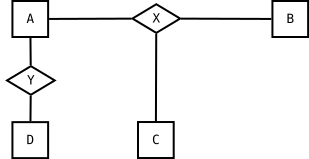
\includegraphics[height=150pt]{resources/er-to-neo4j.pdf}
	\caption{Example conversion of an ER diagram into a \neoj graph}
	
	%Create (a1:A {name: 'A1'}), (b1:B {name: 'B1'}), (b2:B {name: 'B2'}), (c1:C {name: 'C1'}), (c2:C {name: 'C2'}), (d1:D {name: 'D1'}), (d2:D {name: 'D2'}), (x1:X {name: 'X1'}), (x2:X {name: 'X2'}), (a1)-[:XA]->(x1), (x1)-[:XB]->(b1), (x1)-[:XC]->(c1), (a1)-[:Y]->(d1), (a1)-[:Y]->(d2), (a1)-[:XA]->(x2), (x2)-[:XB]->(b2), (x2)-[:XC]->(c2)
	
	\label{fig:example-er-diagram}
\end{figure}

\subsection{\masymos}
\label{sec:background:graph-db:masymos}

This work is mainly based on \masymos, "a graph database for simulation models and associated data" \citep{Henkel2015}, which is implemented using \neoj \citep{Robinson2013}

Since \masymos is developed for "storing and retrieving structural information of biological models" \citep{Henkel2015}, it needs to incorporate mentioned graph representations of simulation networks and an efficient way to query those. Therefore \neoj was the ideal choice, as it works as large property graph, but also "follows fundamental properties of databases, i.e. the ACID principles. \citep{Henkel2015}

The internal schema used by \masymos, as shown in figure \ref{fig:background:graph-db:masymos}, features a \texttt{DOCUMENT} node as standard entry point. This \texttt{DOCUMENT} node represents the actual \xml document and has only one direct child: The \texttt{MODEL} node, which is the entry point for the actual model and represents the \xml root node.

Beyond these two nodes, the schema depends on the format, encoding the imported model. For \sbml the \texttt{MODEL} node is linked to compartments, species, and reactions. Which on the other hand can be linked among each other, expressing relations like reaction reactants and products, or association to a compartment.
Whereby in \cellml the \texttt{MODEL} node links to components, which again contain variables and mathematical expressions, manipulating other variables.

Further semantic annotations, like ontology terms or publication, and author relations, are represented by additional nodes and link to the corresponding ontology term, stored in \neoj, or the interrelated publication or person node. 
Ontology terms are imported according to their hierarchical structure from the \owl representation, which preserves the classification information and therefore allows for searching for abstract terms, but still support traversing to more detailed terms and vice versa.
Commonly imported ontologies are System Biology Ontology\footnote{\url{http://purl.bioontology.org/ontology/SBO}} (SBO), Gene Ontology\footnote{\url{http://purl.bioontology.org/ontology/GO}} (GO), KiSAO\footnote{\url{http://purl.bioontology.org/ontology/KISAO}} and Chebi Ontology\footnote{\url{http://purl.bioontology.org/ontology/CHEBI}}

In addition to explicit links, the graph database back-end of \masymos allows to include implicit links into analysis (those with more than one hop in the graph). Implicit links can link between two models, published by the same person or between model with, common annotations, or even between models using annotations of the same ontology branch.
Further, to allow easy upwards traversal, all relations also feature a common relation to the next higher node in hierarchy, called \texttt{belongs\_to}.

\todo{paragraph about shortcomings}
\begin{figure}[h]
	\centering
	\includegraphics[width=\textwidth]{resources/masymos_struc_figure2.eps}
	\caption{Structure representing \sbml and \cellml models in \masymos. Figure taken from \citealt{Henkel2015}.}
	\label{fig:background:graph-db:masymos}
\end{figure}

\begin{comment}
% following some quotes from the Henkel2015 paper
\begin{itemize}
	\item This work is based on MaSyMoS, "a graph database for simulation models and associated data" \citep{Henkel2015}
	\subitem \citep{Henkel2015} Many models in public databases encode networks that can be represented as graphs
	\subitem \citep{Henkel2015} relational databases were developed for homogeneous, structured data, e.g. numerical data
	\subitem \citep{Henkel2015} Designing a relational representation for these links and keeping the database efficient at the same time are impossible
	
	\item \citep{Henkel2015} MaSyMos is a database based on neo4j for storing and retrieving structural information of biological models
	\subitem \citep{Henkel2015} We chose the graph database Neo4J (25)
	\subitem \citep{Henkel2015} follows the fundamental properties of databases, i.e. the ACID principles
	
	\item \citep{Henkel2015} biological models are represented in heterogenous data structures e.g. networks. Traditional relational databases are build to quickly process highly structured data in tables, therefore they are less efficient in storing and retrieving standard encoded models, due to their highly linked structure
	\subitem \citep{Henkel2015} No unified schema exists for models and meta-data, making it difficult to define a relational database schema
	\subitem \citep{Henkel2015} highly linked models, model entities and meta-data are difficult to represent in a table-based relational database
	\item \masymos data model and structure
	\subitem \citep{Henkel2015} document root node is created for each data item
	\subitem each model is represented by a model node
	\subsubitem entry point for each model import is a document node
	\subitem \citep{Henkel2015} Attached to the model node are annotation nodes, including the reference publication
	\subitem in SBML compartments, species and reactions are linked to the model node
	\subitem in CellML each component is linked to the model node, further containing variables and mathematical relationships to manipulate other variables
	\subsubitem \citep{Henkel2015} component contains vari- ables and mathematical relationships that manipulate those variables
	\subitem Experiment setups are stored under a SEDML node, instead of a model node. In comparison to species, reactions, compartments or components the SEDML node has links to Modelreference nodes, as well as nodes pointing to different model entities used in plots. Nevertheless no processing information is stored in the database.
	\subsubitem \citep{Henkel2015} SEDML node serves as the anchor for an experiment
	\subsubitem \citep{Henkel2015} Modelreference node links the experiment to all Model nodes used in the simulation
	\subsubitem \citep{Henkel2015} do not store the specific processing of a model entity
	\subitem Semantic annotations and cross-references from the models are stored as seperate nodes and linked to the ontology node representing the used ontology term.
	\subsubitem \citep{Henkel2015} Semantic annotations and cross-references
	\subsubitem \citep{Henkel2015} We parse these ontologies and add all concepts and relations as nodes and edges, respectively.
	\subitem ensure an easy traversal upwards, a connection is created from each node of the stored model that points to the parent of the current node. The corresponding edges are named belongsTo]
	\item Linking model related data
	\subitem main advantage to prior mentioned storage in relational databases is the possibility to flexibly link data between different domains. //Henkel et al.// describes 3 different links, which are currently implemented: 1. links between (model) annotations and the corresponding ontology term 2. links between models or model entities and SEDML simulation descriptions or respectively SEDML variables 3. links between model entities in different standard format representation
	\subsubitem \citep{Henkel2015} The main advantage of the previously described concept is its possibility to define flexible links between the data do\item mains)
	\subsubitem \citep{Henkel2015} links between annotations (in SBML, CellML and SED-ML) and ontology concepts)
	\subsubitem \citep{Henkel2015} links between models (in SBML or CellML format) and SED-ML
	\subsubitem \citep{Henkel2015} link is that between a model and a simulation description
	\subsubitem \citep{Henkel2015} links between model entities and SED-ML variables
	\subsubitem \citep{Henkel2015} links between model entities from different model rep- resentation formats
	\subitem \citep{Henkel2015} For each annotation in a model we add an explicit link to the data entry in the ref- erenced bio-ontology
	\subitem This link is shared between all models using this annotation, regardless of the format
	\subitem Further to explicit links (one hop in the graph), MaSyMoS is able to determine implicit links between different models. Those can be established over shared resources like a publication, publication author or annotations with common bio-ontologies. Regarding a publications the database may establish connections based on the likelihood of names by Hemming Distance, resulting in a confidence which can be increased, "" if the entities' annotations match
	\subsubitem \citep{Henkel2015} In addition, we determine implicit links between models of different representation formats
	\subsubitem \citep{Henkel2015} If two models share a publication, the systems can infer implicit links between those entities that are equally named
	\item Implementation
	\subitem MaSyMoS is designed to run as both standalone commandline application with embedded neo4j and as an extension to the neo4j server. Latter is controlled by an unmanaged neo4j plugin providing a RESTful json interface.
	\subitem Same interface also cooperates with the retrieval engine Morre, by providing endpoints to query different search indexes.
	
	\item MaSyMoS project structure
	\subitem The MaSyMoS project is divided into 3 different modules: MaSyMoS-core, Morre and a CLI.
	\subitem The core module contains the logic of the database and communicates directly with neo4j. It consists of routines and a Java API to import models, experiments and ontologies. Further it fetches linked information from common bio-ontologies and manages, updates and queries Lucene indexes.
	\subitem The Command Line Interface (CLI) provides a user interface, to easily interact with the API provided by the core module. It's main purpose was to simplify the development process by skipping the deployment step. Instead it is possible to directly interact with and debug MaSyMoS
	\subitem The Morre module is similiar to the CLI, by providing an way to interact with the core. But instead of providing a user interface, Morre is loaded as neo4j unmanaged extension and exposes a RESTful interface, which can be used to query the Lucene indexes or to push and update models to the database.
\end{itemize}
\end{comment}
\todo{Pictures}


	
	\chapter{Conceptual Architecture}
	\section{Overall system architecture and services}
\begin{itemize}
	\item cf. \ref{fig:system-overview}
	\item \todo{highlight the differences between optimal (proposed) infrstructure and the implementation}
\end{itemize}

\begin{figure}[h]
	\center
	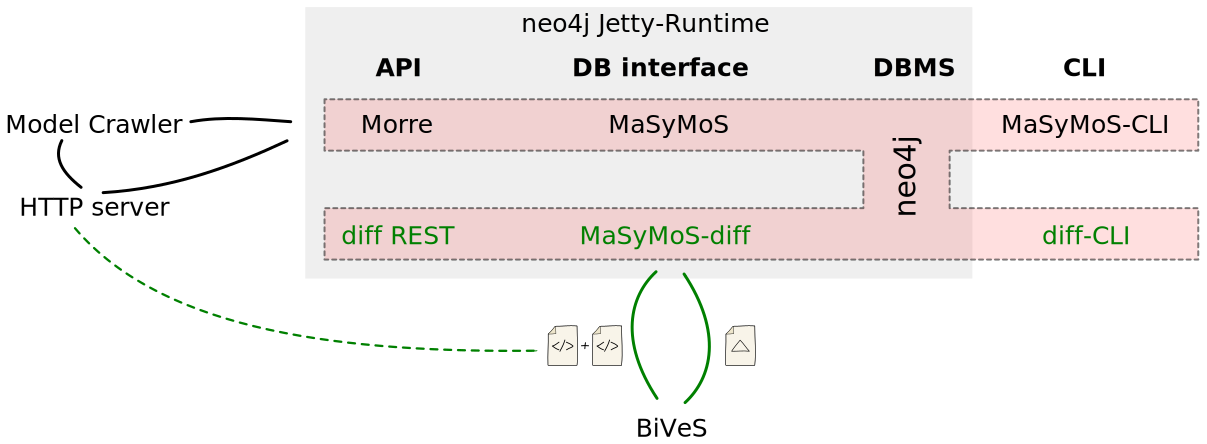
\includegraphics[width=\textwidth]{resources/system-overview-matrix.pdf}
	\caption{Infrastructure overview}
	\label{fig:system-overview}
\end{figure}

\section{Database model and storage decisions}
\begin{itemize}
\item extension to database model cf. \ref{fig:db-model}
	\subitem linking version
	\subitem storing differences
\item decisions on storage model
	\subitem storing each version full (no delta-storag)
	\subitem each version is aware to the search index
	\subitem diff still enables for analysis of changes
	\subitem higher storage consumption
\item extended storage model
\end{itemize}

\begin{figure}[h]
	\includegraphics[width=\textwidth]{resources/db_structure.jpg}
	\caption{Proposed database structure}
	\label{fig:db-model}
\end{figure}

	
	\chapter{Results}
	\todo{what's done from the concept}
\todo{still high-level}
\todo{what problem is solved?}

solved:
"A model VCS should be tailored to existing model representation formats, which are typically XML and RDF based. It should furthermore reflect the temporal evolution of a model and present model changes to the users." \citep{Waltemath2013}
	
	\chapter{Implementation of the Prototype}
	% !TeX spellcheck = en_US
\todo{concrete, low-level stuff}
\todo{what was used, version numbers, etc.}
\todo{pretty short, every subproject gets a section}
\todo{add figure showing differences of concept and implementation, regarding figure \ref{fig:system-overview}}

\section{\modelcrawler}
	\label{sec:impl:modelcrawler}
	The \modelcrawler is not directly product of this project, but was developed by me in course of my work as student assistant at the department for \sysbio and Bioinformatics. However, it is mentioned here, since it responsible for creating the repository containing all original files, which is one of the integral parts of the presented concept (cf. Section \ref{sec:concept:filestorage}).
	
	The version described here is 0.0.4 mark2, commit \texttt{abb63db}. Overall the function of the \modelcrawler is relatively simplistic and was designed, so it could be ran incrementally, gradually crawling only (a limited amount) new versions. Each pass through therefore consists of two steps: First the databases are crawled, the new versions or releases are downloaded and stored in said file structure.
	Second the \modelcrawler pushes all new model versions to \masymos, theoretically allowing for improved write speed, due to transaction management. However, the main reason for splitting the actions is better error recovery. By keeping the time of write operations on the database short and not running any other concurrent task, the probability of interruptions is minimized. This means, when the \modelcrawler fails, due to bugs in the implementation, changes in the API, or other external influences (e.g. Java Heap Exceptions), the database does not get inconsistent. This is guaranteed, because ahead of inserting data, the \modelcrawler ensures all data is valid and consistent.
	
	However the first step, downloading all new versions, heavily depends on the to be crawled database.
	In case of \emph{BioModels Database} all not already crawled release are downloaded from the FTP server with Apache Commons Net library version 3.3, unpacked with Apache Commons Compress version 1.9. Consequently each \xml file is analyzed.
	If a file with equal name or BioModels ID is already indexed in \masymos, the SHA-1 hash of the files is calculated. If this differs from the file hash of the latest version in \masymos, a new version is assumed.
	
	This process is easier for \emph{PMR2}, since it already uses git repositories to keep track of versions/revisions of models. Therefore it is just a matter of interfacing the \rest API with Apache HttpClient 4.3 and FasterXMLs Jackson 2.5.1, to list all publicly available repositories. These repositories are then cloned or pulled with eclipses JGit library, version 3.7.0. Following all commits are iterated, and all newer than the latest version in \masymos are considered new.

	Since the \modelcrawler relies on the \masymos database, to identify already existing versions, it can operate stateless between different pass throughs. However, it keeps separately track of already downloaded BioModels releases and all previously cloned git repositories in order to minimize the amount of data, which needs to be transfered.

\section{Extension to the \masymos core}
	\label{sec:impl:masymos}
	\begin{itemize}
		\item generic ontology import for COMODI
		\item some helper methods/functions
	\end{itemize}

\section{\masymos diff plugin}
	\label{sec:impl:diff}
	\begin{itemize}
		\item interaction with \bives and neo4j
		\item problems with Transaction rollback in actually successfull transactions
	\end{itemize}

\section{\rest interface and scheduling}
	\label{sec:impl:rest}
	\begin{itemize}
		\item \rest interface for requesting diffs
		\item time based trigger for generating diffs for new versions
	\end{itemize}


	
	\chapter{Discussion}
	% !TeX spellcheck = en_US

Opposed to traditional VCSs (cf. Section \ref{sec:background:manage-versions:traditional-vcs}) the system presented in this thesis is not meant to support developers during the development process, since \masymos is originally developed as a search index (cf. Section \ref{sec:background:graph-db:masymos}).
Rather it is designed to assist other developers, who want to build upon existing models.
This shift in focus, allows to analyze and organize already published models, as well as it does not need any interaction from the modelers. The lacking need of user cooperation might help to building up the data stock quicker, but also limits the amount of meta information.
However, by not relying on anybody specifically using this system, I was able to quickly accumulate a large test set, as mentioned in the Results (cf. Chapter \ref{sec:results}).

Being an analytic platform and not a day-to-day tool sets different constraints. For instance access time becomes more crucial, whereby consumed drive space is less a concern.
My implementation takes full advantage of this loosened space restriction.
The storage structure, I decided on, is not optimized by using an efficient reverse-delta storage as traditional VCS would do (cf. Section \ref{sec:background:manage-versions:traditional-vcs}).
Instead each model is stored completely for multiple reasons: it allows for a very lose coupling to the base \masymos implementation, meaning the diff-extension is additive to the features of \masymos and does not require for intrusive changes of the code base.
Further the core functionality of \masymos is not disturbed and provides a full text and structural search index entry for each version of a model.
Therefore every single model version is treated as distinct model, resulting in easier structural analyses per model version and less expensive operations on the indexes, when inserting a new model version.

On the downside, the complete storage of each model increases the database size significantly. But to keep the scope of this work concise and the prototype implementation of reasonable complexity, I focused on a good data interlinkage and less on an efficient storage model.

This decision might show some drawbacks with a growing amount of models and versions.
First issue to consider would be higher storage consumption, but also slower query execution should be considered.
Second, \bives creates multiple changes, which have a single common source. For instance adding a \emph{species} in \sbml will result in at least five changes. These include the insertion of the element itself and the insertion of the attributes \texttt{id}, \texttt{name}, \texttt{initialConcentration}, and \texttt{compartment} reference.
Storing this many changes encoding similar information increases the overall size dramatically.

A way to reduce the overhead of storing deltas could be to calculate them only on demand. This would, however, reduce the database to a cache for \bives and eliminate all possibilities to analyze changes in large scale.

Both issues could also be improved or even solved by using a database design with less redundancies. This means in relation to the first point, to implement the database as reverse-delta storage, accepting all the mentioned drawbacks.
In the second issue less redundancies could be archived by grouping changes which clearly share the same origin.

Grouping changes will inevitably lead to less accurate annotation with the \comodi ontology, which on the other hand will limit the use in analysis and statistics of changes. 
Then again, currently the \comodi ontology is only partly used in this project. The \texttt{Reason} and \texttt{Intention} branches (cf. Section \ref{sec:background:onto:comodi}) are not linked from changes, because they aim to explain the cause and purpose of a change. These aspects are hard to determine automatically. Therefore \bives is not capable of using these annotations automatically.
To integrate \texttt{Reason} and \texttt{Intention} in the annotations, further information would need to be processed. This could be archived by user input, either from demanding formalized annotations or by text mining commit messages. 
Both are a imaginable features for a version of this database project adjusted for the use as personal VCS.
Mentioned information could also be conceived by coupling this project with an existing VCS like Git or an data sharing platform like SEEK\footnote{\url{http://seek4science.org/}}.

Concluding, I believe, that the basic design investigated in this thesis has the potential to help solving the essential problem of reproducibility. The database design provides a solid foundation to increase transparency and therefore reproducibility. It allows users and third party tools to explore the evolution of a model with all external links \masymos already provides. In addition with \comodi-annotations common changes or trends can be detected.
Further search engines front-ends could suggest which version matches best the requirements of the user, instead of only returning the newest version. These requirements may be a specific species or compatibility to a \sedml script or another model.

At last it is important to point out, that 

%All in all is this work just as good as the supplied data, therefore it is important to facilitate cooperations and interlink more and more open data.
\todo{add point about not being another bio database/repository}

\todo{find a nice(r) ending?}
\begin{comment}
\todo{incorporate former outlook section}
\begin{itemize}
	\item outlook
	\subitem Improving search index with metrics on how much impact a change had to the search criteria
	\subsubitem "Incremental Query Evaluation. When a user has a standing query against a time-varying data source, a change-detection tool can provide the query engine the delta data on which the query will be re-evaluated. Thus, the user doesn’t receive old results and the query engine avoids repeated work. Since the delta data is usually much smaller than the original data, query evaluation will also be much faster." \citep{Wang2003}
	\subitem detecting similar changes on different models
\end{itemize}
\end{comment}

\begin{comment}
\begin{itemize}
	\item Benchmarks/stats on database
		\subitem additional overhead (nodes/relations increase)
	\item How to improve database/reduce overhead
	\item 2 branches of \comodi unused
		\subitem because of automatic generation
		\subitem reason and intention not able to be automatically determined
		\subitem possible extension?
\end{itemize}
\end{comment}
	
	\chapter{Outlook}
	
\begin{itemize}
	\item Improving search index with metrics on how much impact a change had to the search criteria
		\subitem "Incremental Query Evaluation. When a user has a standing query against a time-varying data source, a change-detection tool can provide the query engine the delta data on which the query will be re-evaluated. Thus, the user doesn’t receive old results and the query engine avoids repeated work. Since the delta data is usually much smaller than the original data, query evaluation will also be much faster." \citep{Wang2003}
	\item detecting similar changes on different models
\end{itemize}

	
	%\bibliography{ba-thesis.bib}
	\bibliography{zotero.bib}
	\bibliographystyle{apalike}
	
	\begin{appendix}
		\listoffigures
		
		\chapter*{Appendix}
		%% !TeX spellcheck = en_US

% some nice styling for code listings
\definecolor{mygreen}{rgb}{0,0.6,0}
\definecolor{mygray}{rgb}{0.5,0.5,0.5}
\definecolor{mymauve}{rgb}{0.58,0,0.82}
\definecolor{lightgray}{rgb}{0.97,0.97,0.97}

\lstset{ %
	backgroundcolor=\color{lightgray},   % choose the background color; you must add \usepackage{color} or \usepackage{xcolor}
	basicstyle=\footnotesize,        % the size of the fonts that are used for the code
	breakatwhitespace=false,         % sets if automatic breaks should only happen at whitespace
	breaklines=true,                 % sets automatic line breaking
	captionpos=b,                    % sets the caption-position to bottom
	commentstyle=\color{mygreen},    % comment style
	deletekeywords={...},            % if you want to delete keywords from the given language
	escapeinside={\%*}{*)},          % if you want to add LaTeX within your code
	extendedchars=true,              % lets you use non-ASCII characters; for 8-bits encodings only, does not work with UTF-8
	frame=no,	                   % adds a frame around the code
	keepspaces=true,                 % keeps spaces in text, useful for keeping indentation of code (possibly needs columns=flexible)
	%keywordstyle=\color{blue},       % keyword style
	keywordstyle={},
	language=Octave,                 % the language of the code
	otherkeywords={*,...},           % if you want to add more keywords to the set
	numbers=left,                    % where to put the line-numbers; possible values are (none, left, right)
	numbersep=5pt,                   % how far the line-numbers are from the code
	numberstyle=\tiny\color{mygray}, % the style that is used for the line-numbers
	rulecolor=\color{black},         % if not set, the frame-color may be changed on line-breaks within not-black text (e.g. comments (green here))
	showspaces=false,                % show spaces everywhere adding particular underscores; it overrides 'showstringspaces'
	showstringspaces=false,          % underline spaces within strings only
	showtabs=false,                  % show tabs within strings adding particular underscores
	stepnumber=2,                    % the step between two line-numbers. If it's 1, each line will be numbered
	stringstyle=\color{mymauve},     % string literal style
	tabsize=2,	                   % sets default tabsize to 2 spaces
	title=\lstname                   % show the filename of files included with \lstinputlisting; also try caption instead of title
}

% helper for importing csv files with underscores
\newcommand{\expScore}{%
	\expandafter\expandafter\expandafter
	\detokenize
	\expandafter\expandafter\expandafter
}

\chapter{Simple demo \sbml models}
\section{Simple demo SBML version1}
\label{sec:appendix:simple-demo:v1}
\lstinputlisting[language=XML]{../supplementary/demo-sbml-simple/version1.xml}
\pagebreak

\section{Simple demo SBML version2}
\label{sec:appendix:simple-demo:v2}
\lstinputlisting[language=XML]{../supplementary/demo-sbml-simple/version2.xml}
\pagebreak

\section[Render of a Delta]{Complete render of the delta graph network}
\begin{figure}[H]
	\centering
	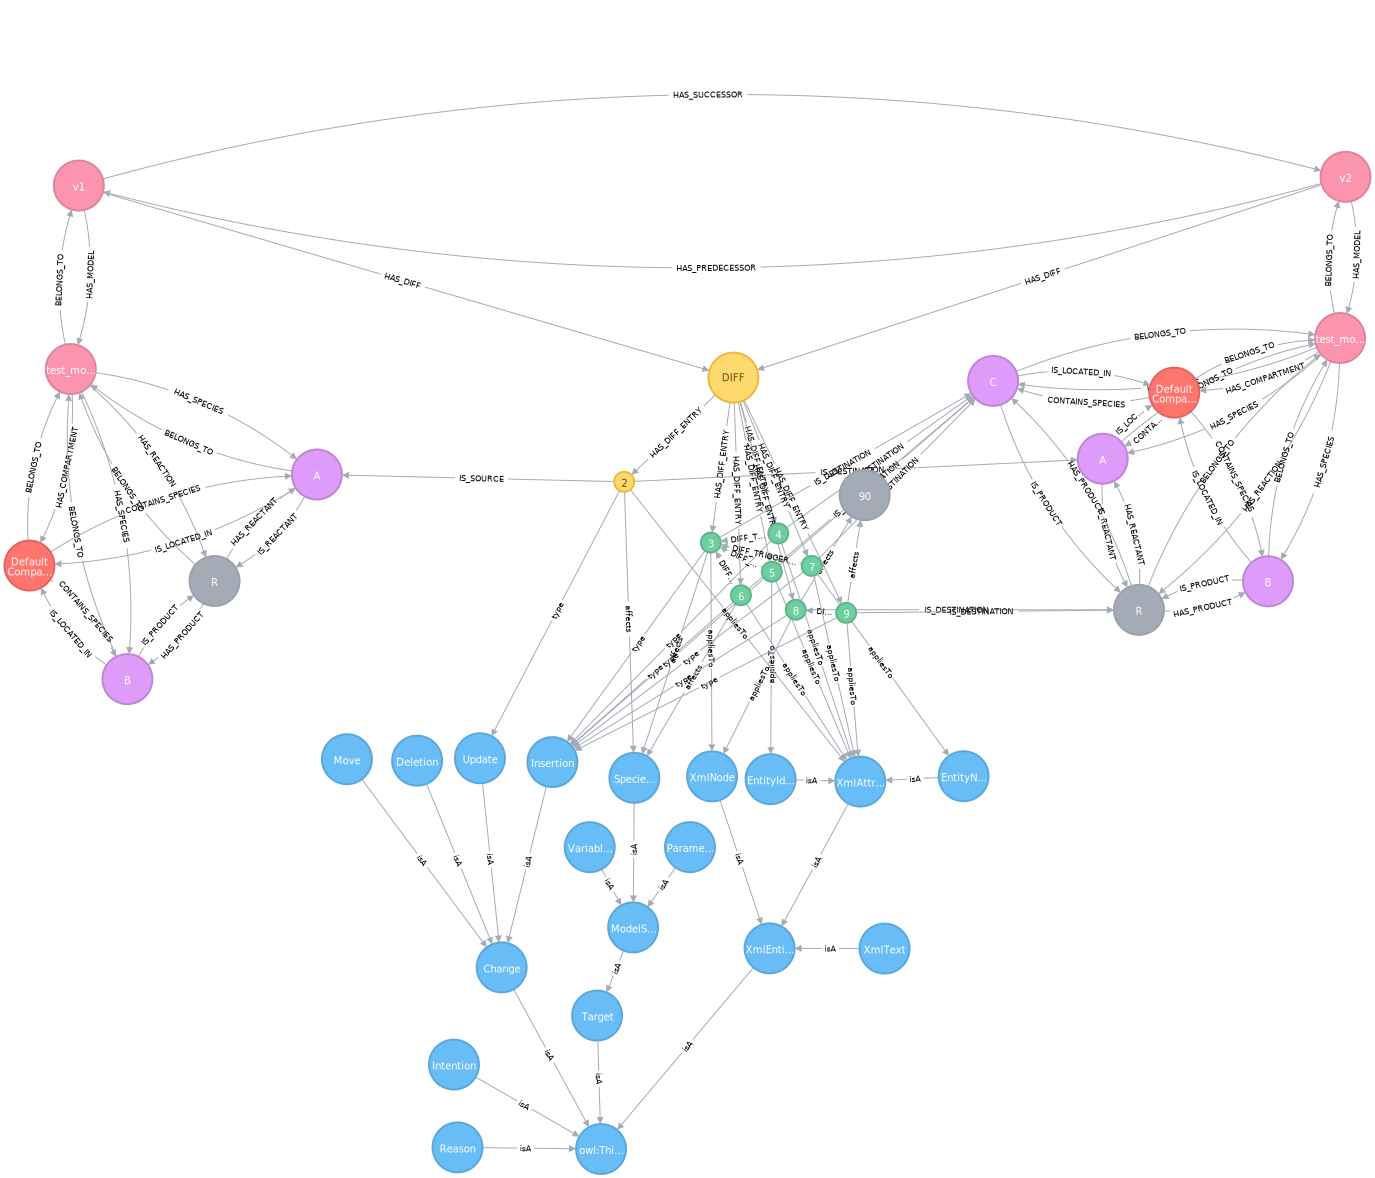
\includegraphics[width=\textwidth]{resources/neo4j-renders/demo-sbml-simple-diff-complete.pdf}
	\caption[\neoj graph representation of a delta between two demo models]{\neoj graph representation of a delta between two demo models. This is the full version of the simplified delta shown in Figure \ref{fig:results:simple-diff}}
	\label{fig:appendix:demo-sbml-simple-diff}
\end{figure}

\chapter{Representation of \comodi in \masymos}
\begin{figure}[H]
	\centering
	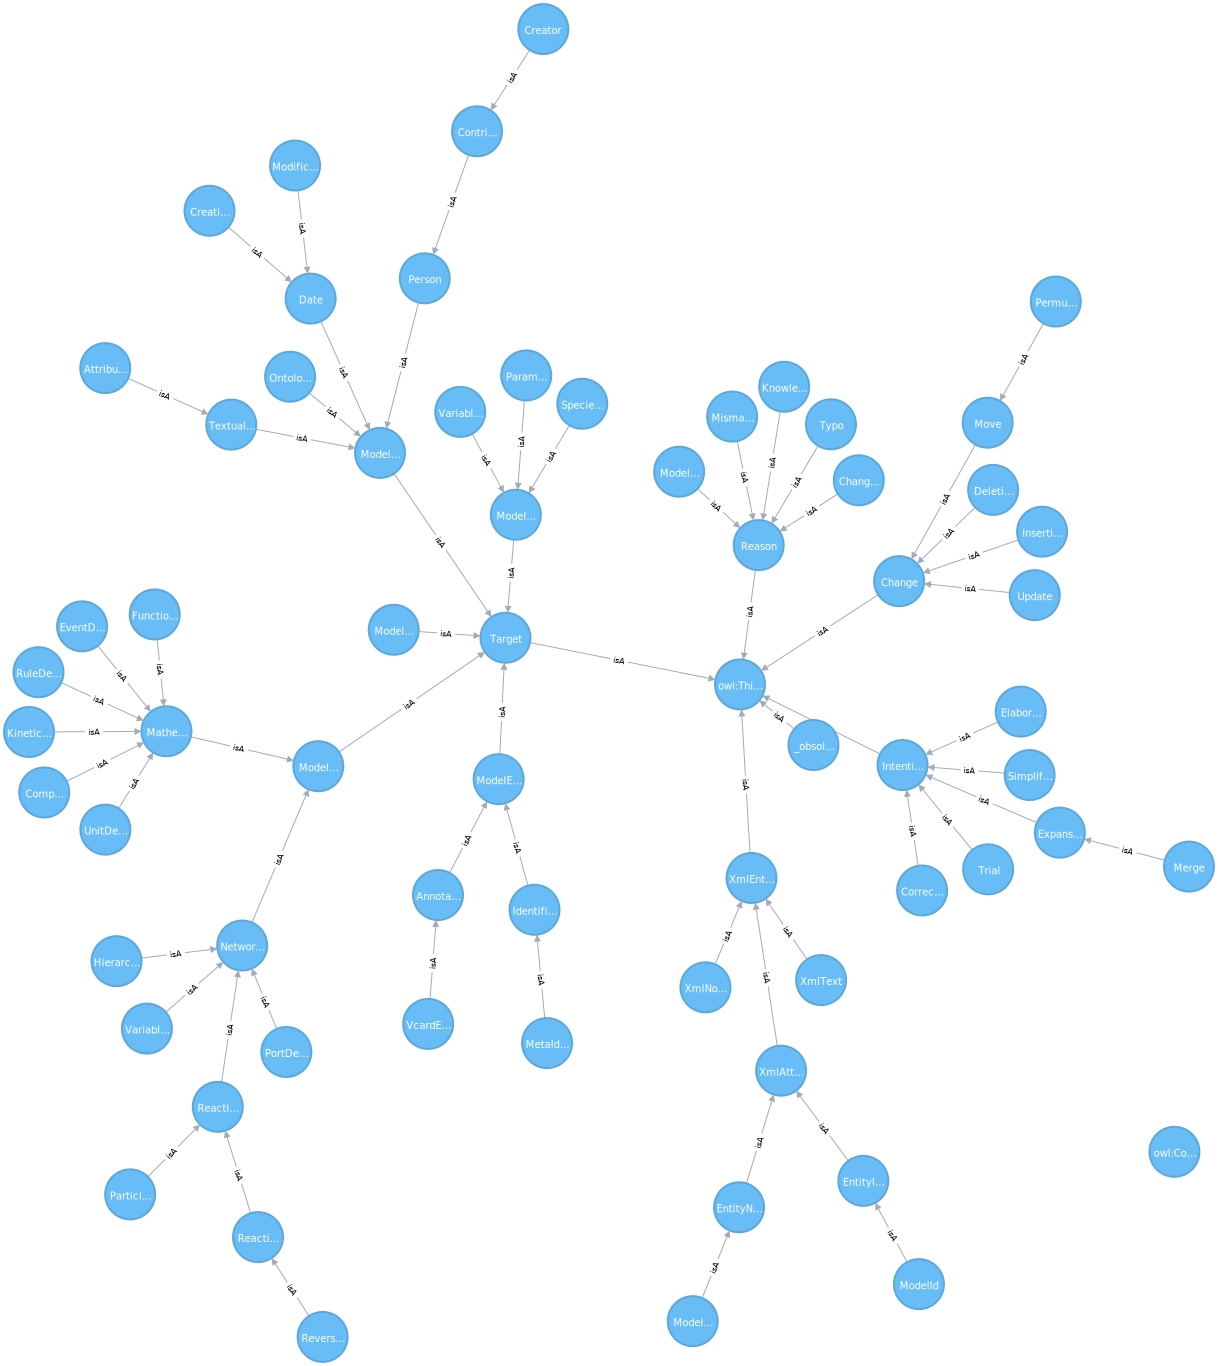
\includegraphics[width=\textwidth,height=0.5\textheight,keepaspectratio]{resources/neo4j-renders/comodi.pdf}
	\caption[Representation of \comodi in \masymos/\neoj]{Representation of \comodi in \masymos/\neoj. For the exact network refer to the documentation Figure \ref{fig:background:onto:comodi}}
	\label{fig:appendix:neo4j-comodi}
	\todo{make text larger/more readable?}
\end{figure}

\chapter{Overview of Node- and Relationship types}
\chaptermark{Node- and Relationship types}
\label{sec:appendix:meta-map}
\todo{write introduction thingy, where these numbers are coming from}

\section{Graphical Overview}
\begin{figure}[H]
	\centering
	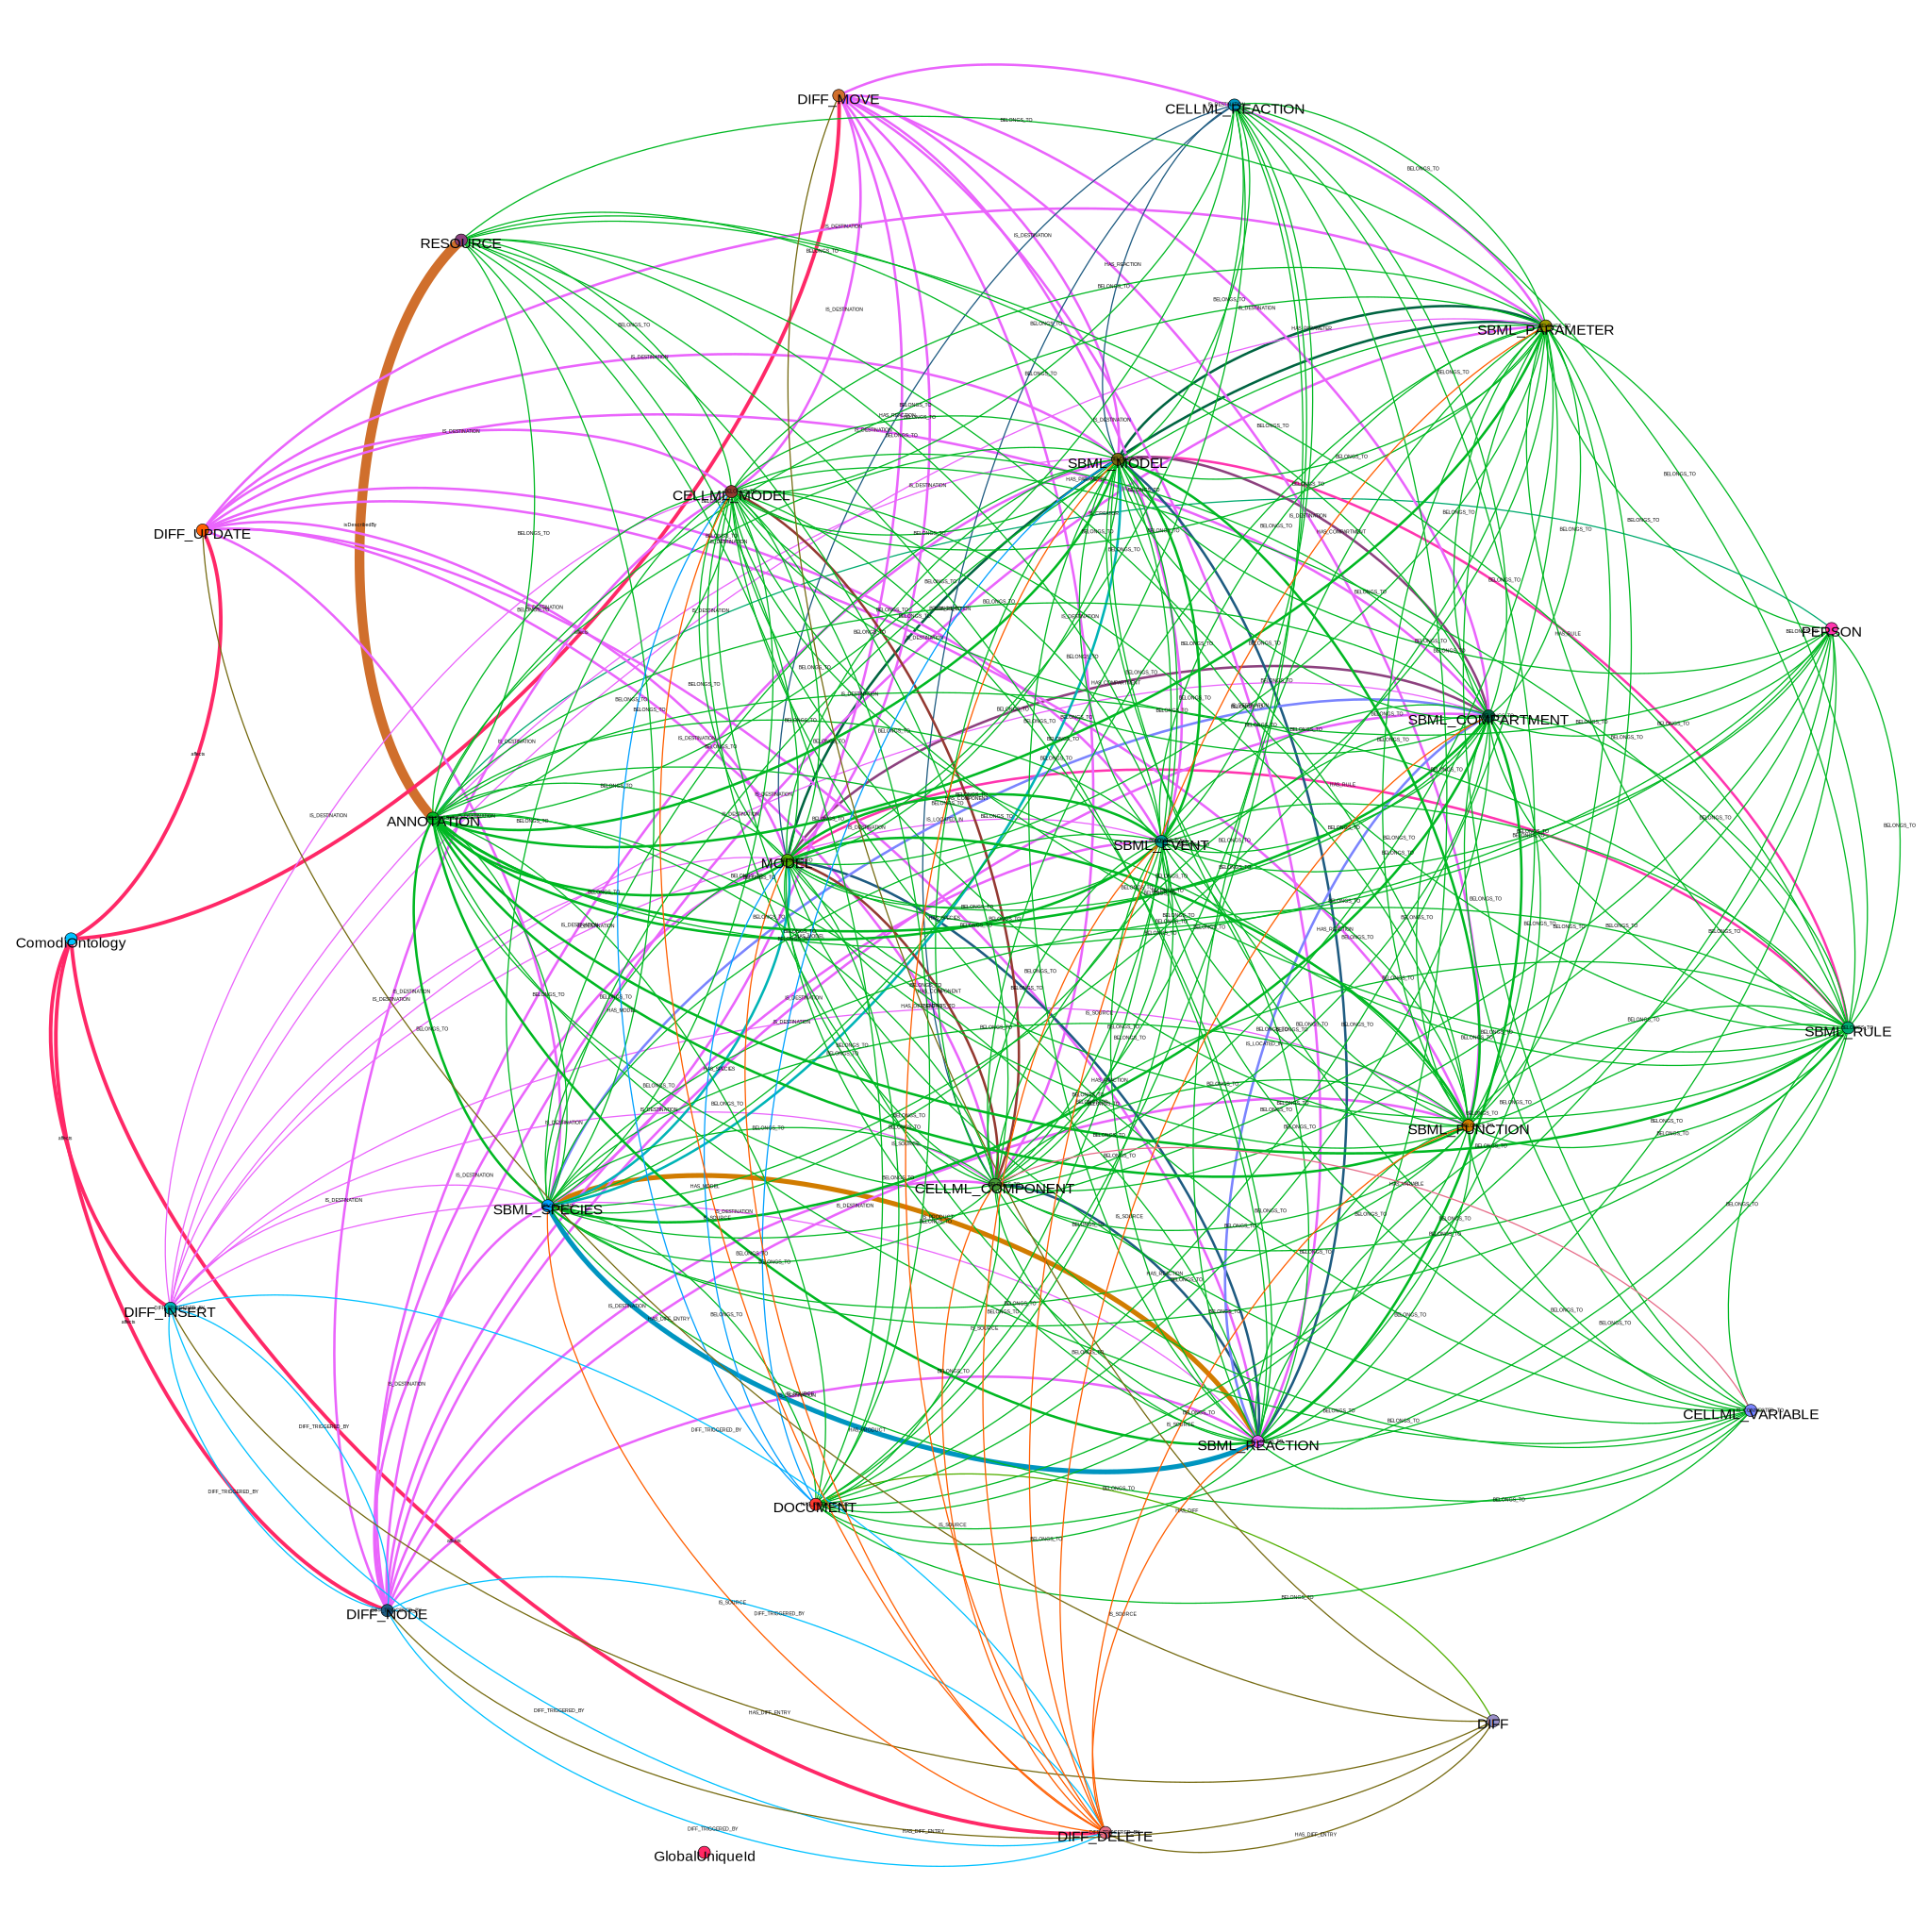
\includegraphics[width=\textwidth,height=0.5\textheight,keepaspectratio]{resources/neo4j-renders/large-test-meta-graph.pdf}
	\caption{Overview of all used node types and relations between them}
	\label{fig:appendix:meta-graph}
\end{figure}

\section{List of all used Node types}
\begin{longtable}{ l r }
	\hline \bfseries Node Label & \bfseries No. of occurrence \\\hline \endhead
	\csvreader[] %
	{resources/neo4j-renders/large-test-meta-graph-nodes.csv}{label=\nodeLabel,count=\count} %
	{\small \texttt{\expScore{\nodeLabel}} & \expScore{\count} \\} %
	%\hline
\end{longtable}

\section{List of all used Relationship types}
\begin{longtable}{ l c r }
	\hline \bfseries Source Node Label & \bfseries Relationship Type & \bfseries Destination Node Label \\\hline \endhead %
	\csvreader[]{resources/neo4j-renders/large-test-meta-graph-edges-expanded.csv}{Source=\sourceNode,Target=\targetNode,label=\relLabel} %
	{\texttt{\expScore{\sourceNode}} & \texttt{\expScore{\relLabel}} & \texttt{\expScore{\targetNode}} \\} %
	%\hline
\end{longtable}

\chapter{Compiling and Building the Prototype Implementation}
\chaptermark{Compiling and Building}

\section{Requirements and Dependencies}
Before attempting to compile and build the source, please make sure that following software packages are installed and working: \texttt{Git}, \texttt{JDK 1.8}, \texttt{Apache Maven 3}, \texttt{build-essentials}, \texttt{wget}, \texttt{curl}, \texttt{Python 3}, and \texttt{pip for Python 3}.

All described steps were developed and tested on \texttt{Linux 4.7.0-1-amd64 \#1 SMP Debian 4.7.8-1 (2016-10-19) x86\_64 GNU/Linux}. Alternative platforms might need adjustments to the build scripts or steps.

\section{Compiling and Building the Database}
% set some new settings for listings
\lstset{
	language=Bash,
	breaklines=true,
	breakatwhitespace=true,
	numbers=none,
	frame=single,
	framerule=0pt,
	belowskip=-24pt,
	aboveskip=5pt,
	basicstyle=\footnotesize\ttfamily,
	stringstyle={},
}

\begin{enumerate}
	\item Clone the repository from GitHub. This step can be skipped, if the material from the attached disc is used.
	\begin{enumerate}
		\item Open a terminal and navigate to a drive with at least 1GB of free disc space.
		\item Clone the main repository from GitHub:
\begin{lstlisting}
git clone git@github.com:FreakyBytes/bachelor-thesis.git
\end{lstlisting}
		\item Navigate into the newly cloned repository:
\begin{lstlisting}
cd bachelor-thesis
\end{lstlisting}
		\item Clone all git submodules:
\begin{lstlisting}
git submodule init
git submodule update
\end{lstlisting}
	\end{enumerate}

	\item Change into the \texttt{source} directory:
\begin{lstlisting}
cd source
\end{lstlisting}

	\item Start the build process:
\begin{lstlisting}
make all neo4j
\end{lstlisting}
		This command will invoke the build process for each subproject using Maven, also it will download, extract, and configure \neoj with all required dependencies. The resulting distribution can be found in the \texttt{neo4j} folder.
\end{enumerate}

\section{Populating the Database with Test Data}

\begin{enumerate}
	\item Open a terminal and navigate into the \texttt{source} directory, if not already done.
\begin{lstlisting}
cd source
\end{lstlisting}

	\item Make sure, that \neoj is not running:
\begin{lstlisting}
cd neo4j
bin/neo4j stop
cd ..
\end{lstlisting}

	\item Import the \comodi ontology using the \masymos-CLI:
\begin{lstlisting}
java -cp masymos-cli/target/masymos-cli-0.9.1.jar de.unirostock.sems.masymos.main.MainExtractor -dbPath ./neo4j/data/databases/graph.db -type owl -ontology ComodiOntology -directory ./COMODI/ontology/comodi.owl
\end{lstlisting}

	\item Start \neoj:
\begin{lstlisting}
cd neo4j
bin/neo4j start
\end{lstlisting}

	\item Change into the \texttt{ba-scripts} directory.
\begin{lstlisting}
cd ../../ba-scripts
\end{lstlisting}

	\item Install all \texttt{Python} dependencies, required for the \texttt{push2masymos} script:
\begin{lstlisting}
pip install -r requirements.txt
\end{lstlisting}

	\item Fill the database with test models, using the \texttt{push2masymos} script:
\begin{lstlisting}
python push2masymos.py --log=DEBUG -d test_models.yaml
\end{lstlisting}
	After all models are pushed the script will remain running and therefore continue to serve the model files via HTTP. This is important because the files need to be accessible in order to generate the diffs.

	\item Open a new terminal and trigger the diff generation using the \rest endpoint:
\begin{lstlisting}
curl -X POST http://localhost:7474/diff/service/trigger
\end{lstlisting}
	
	\item The progress can be observed using the \texttt{/stats} and \texttt{/status} endpoint:
\begin{lstlisting}
watch -n 10 "curl -X GET http://localhost:7474/diff/service/stats 2>/dev/null | python -m json.tool ; curl -X GET http://localhost:7474/diff/service/status 2>/dev/null | python -m json.tool"
\end{lstlisting}

	\item The \neoj web-interface is now available under:\\ \url{http://localhost:7474/browser/}
\end{enumerate}


	\end{appendix}
\end{document}
